%Made By Thomas Debelle
\documentclass{report}
\usepackage[a4paper, total={6in, 9in}]{geometry}
\usepackage[utf8]{inputenc}
\usepackage[francais]{babel}
\usepackage{graphicx}
\usepackage{graphics}
\usepackage[T1]{fontenc}
\usepackage{amsmath}
\usepackage{hyperref}
\usepackage{amssymb}
\usepackage{listings}
\usepackage{xcolor}
\usepackage{array}
\usepackage{float}
\usepackage{amsfonts}
\usepackage{fancyhdr}
\usepackage{titlesec}
\usepackage{xparse}
\usepackage{wrapfig}

\hypersetup{
    colorlinks=true,
    linkcolor=black,
    filecolor=magenta,
    urlcolor=cyan,
    pdftitle={Overleaf Example},
    pdfpagemode=FullScreen,
    }
\begin{document}


\begin{titlepage}
    \begin{figure}
        
\includegraphics[height = 2cm]{UCL_Logo.png}
        \label{fig:my_label}
    \end{figure}

    \hspace*{100cm}
    \centering
    \vspace*{7cm}

    {\Huge \textbf{Résumé de LELEC1370}}\\
    \vspace*{0.25cm}
    compilation du \today\\
    \vspace*{0.25cm}
    \Large{Thomas Debelle}\\

    \vspace*{9.5cm}
    {\Large Juin 2023}
\end{titlepage}


\tableofcontents
\newpage

\section*{Préface}

Bonjour à toi !\\

Cette synthèse recueille toutes les informations importantes données au cours, pendant les séances de tp et est amélioré grâce au note du Syllabus. Elle ne remplace pas le cours donc écoutez bien les conseils et potentielles astuces que les professeurs peuvent vous donner. Notre synthèse est plus une aide qui on l'espère vous sera à toutes et tous utiles.\\

Elle a été réalisée par toutes les personnes que tu vois mentionné. Si jamais cette synthèse a une faute, manque de précision, typo ou n'est pas à jour par rapport à la matière actuelle ou bien que tu veux simplement contribuer en y apportant ta connaissance ? Rien de plus simple ! Améliore la en te rendant \href{http://www.github.com/Tfloow/Q4_EPL}{ici} où tu trouveras toutes les infos pour mettre ce document à jour. (\textit{en plus tu auras ton nom en gros ici et sur la page du github})\\

Nous espérons que cette synthèse te sera utile d'une quelconque manière ! Bonne lecture et bonne étude.


\chapter{Cours 1}
\section{Les bases}

Tout d'abord, il existe 2 types de courant appelé \textbf{Direct Current} ou \textit{DC} et \textbf{Alternating Current} ou \textit{AC}. Le courant direct est continu tandis que le courant \textit{AC} varie dans le temps comme montré ci-contre.\\
\begin{figure}[H]
	\centering
	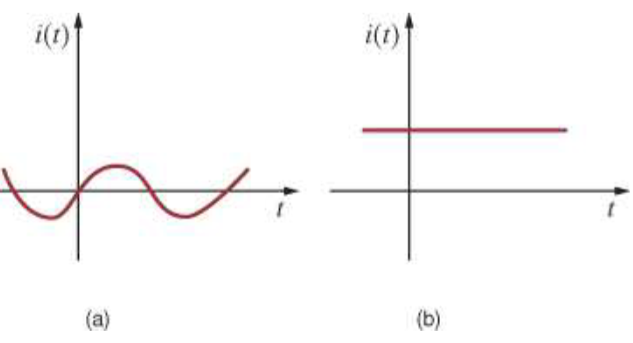
\includegraphics[width=.3\textwidth]{img/ACDC.png}
	\caption{Gauche: courant AC \quad Droite: courant DC}
\end{figure}
La tension vaut la variation d'énergie selon la charge ou autrement dit: 
\begin{equation}
v = \frac{dw}{dq}
\end{equation}
La puissance vaut la tension par le courant ou:
\begin{equation} \label{eqn:p}
p = vi = \frac{dw}{dq}\frac{dq}{dt}
\end{equation}
Finalement, l'énergie est une différence de puissance en fonction du temps:
\begin{equation}
\Delta w = \int_{t_1}^{t_2}p dt = \int_{t_1}^{t_2} vi dt
\end{equation}
Quelques conventions:
\begin{itemize}
\item Source de tension nulle = court circuit
\item Source de courant nulle = circuit ouvert
\item Le sens du courant "rentre" dans la borne + d'un générateur de tension.
\end{itemize}
\subsubsection{Puissance dissipée}
Pour connaitre la puissance dissipée dans une résistance, on utilise d'abord la formule fondamentale d'une résistance:
\begin{equation}
v(t) = R i(t)
\end{equation}
Ainsi, en utilisant \ref{eqn:p} on trouve:
\begin{equation} \label{eqn:pr}
p(t) = vi(t) = \frac{v^2(t)}{R} = Ri^2(t)
\end{equation}

\subsubsection{Loi des noeuds de Kirchoff}
La somme des courants de tous les noeuds a pour résultat 0. Autrement dit, tout courant qui apparait disparait quelque part.

\subsubsection{Loi des mailles de Kirchoff}
Dans un circuit électrique, on peut dessiner des \textit{mailles} ou des sortes de carrés. En tournant dans un sens, on fait la somme des tensions (\textit{faire attention au sens des tensions}) on obtient une somme nulle.

\subsubsection{Sources multiples - Diviseur de tension}
On peut simplifier un circuit et sommer des sources de tension en additionnant leur tension. On utilise également la règle des diviseurs de tension pour les résistances:
\begin{equation}
\begin{cases}
\parallel \rightarrow R_{new} = \frac{1}{\frac{1}{R_1}+\frac{1}{R_2}}\\
\text{série} \rightarrow R_{new} = R_1 + R_2
\end{cases}
\end{equation}

\subsubsection{Mise en parallèle et sources multiples}
Les sources de courant en parallèle peuvent être sommé pour les simplifier et n'en avoir qu'une seule source de courant.

\subsubsection{Équivalent Thévenin Norton}
On peut simplifier une alimentation d'un circuit via les circuits de Thévenin et Norton. Thévenin est composé d'une source de tension et d'une résistance en série tandis que Norton a une source de courant et une résistance en parallèle.\\
Les choses importantes à noter sont:
\begin{equation}
\begin{cases}
R_{Th} = R_{No}\\
I_{sc} = \frac{V_{R}}{R_{Th}}\\
v_{oc} = R_{Th}i_{sc}
\end{cases}
\end{equation}
 
\begin{figure}[H]
\centering
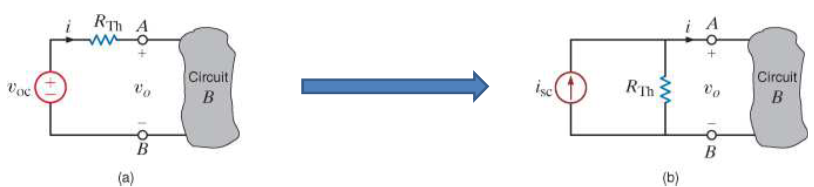
\includegraphics[width = 10cm]{img/ThNo.png}
\caption{Illustration du passage de Thévenin à Norton}
\end{figure}
Pour trouver la résistance $R_{Th}$ on met en \textit{court-circuit} les générateurs de tensions et en \textit{circuit ouvert} les générateurs de courant. Ensuite, on enlève la résistance et on regarde à ses bornes les \textit{résistances} et on trouve donc \textit{l'équivalent des résistances}. On peut faire cela uniquement avec des générateurs \textbf{non commandés}.\\

Pour trouver le \textit{courant de Norton} et la \textit{tension de Thévenin} (on est \textbf{obligé} de passer par cette étape en premier avec des \textit{sources commandées}). Pour \textit{Thévenin} on met notre résistance en \textit{circuit ouvert} et on trouve le voltage à ses bornes.\\
Pour \textit{Norton} on met notre résistance en \textit{court-circuit} et on trouve le courant circulant dans ce fil.

\subsubsection{Conseil Norton Thévenin}
Lorsqu'on travaille avec des courants, on utilise la loi des \textit{noeuds} et une fois qu'on a toutes les équations, on utilise la loi des \textit{mailles} qui permet d'utiliser nos courants et tout simplifier.\\

\subsubsection{Dualité étoiles-triangle}
Dans un circuit électrique, on peut faire face à des arrangements de résistances en \textit{triangle} qui sont compliqués à transformer en \textit{résistance équivalente}. 
\begin{figure}[H]
\centering
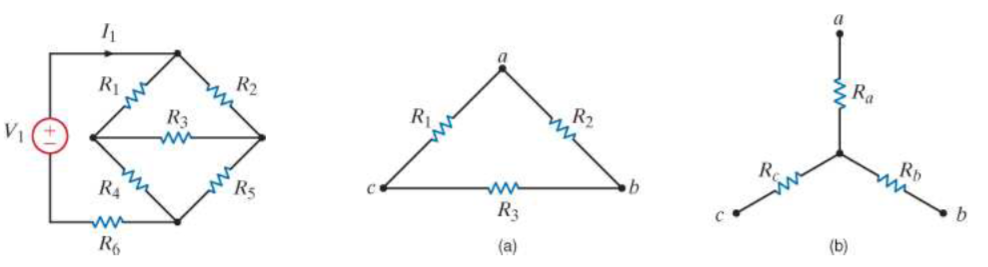
\includegraphics[width=7cm]{img/triangleEtoile.png}
\caption{Passage d'une forme de triangle à une forme d'étoiles}
\end{figure}



\chapter{Cours 2}
\section{Suite des bases}
\subsubsection{Thévenin avec sources dépendantes}
Pour trouver $R_{Th}$ on va rajouter au borne connectant l'autre circuit une source de tension. Puis on détermine les tensions à borne ouverte et le courant en \textit{court-circuit}.

\subsubsection{Transfert maximal de puissance}
Pour trouver la puissance maximale dans une résistance, on peut faire varier le courant et donc le voltage. Ici, on a réalisé un diviseur résistif très simple pour démontrer la formule de puissance de résistance donné par \ref{eqn:pr}, on obtient donc ceci dans notre circuit:
\begin{equation}
\frac{\partial}{\partial R_2} \biggl(\frac{V^2 R_2}{(R_1 + R_2)^2}\biggl) = 0
\end{equation}

\begin{figure}[H]
\centering
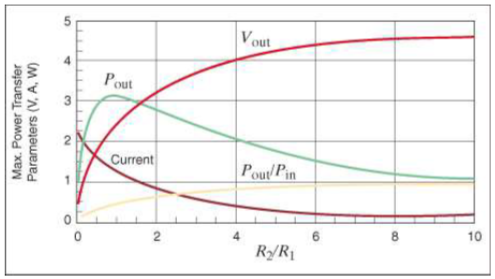
\includegraphics[width=6.5cm]{img/maxPuissance.png}
\caption{Graphique montrant l'évolution de la puissance dans une résistance}
\end{figure}

\subsubsection{Le quadripole à 2 accès}
\begin{wrapfigure}{r}{.45\textwidth}
\centering
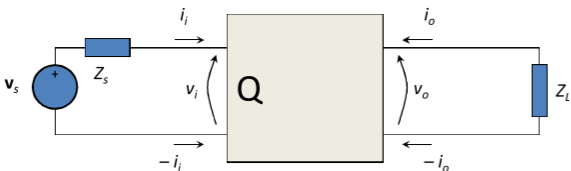
\includegraphics[width=6.5cm]{img/quadri2.png}
\caption{Schéma classique d'un quadripole à 2 accès}
\end{wrapfigure}
Le quadripole à 2 accès se reposent sur 2 principes, il faut qu'il n'y ait aucune source indépendante interne $\rightarrow$ donc passif. Il faut également n'avoir que 2 accès, c'est à dire que la somme des entrées est nulle. Pour simplifier, il faut qu'on ait une entrée et sortie comprenant le même courant (voir schéma ci-contre).\\
Le but de cette représentation est une simplification de circuit. De plus, même si ce circuit n'est pas linéaire, on fait des petites variations autour d'une valeur rendant approximativement le circuit linéaire.\\

Ce type de quadripole peut être réalisé de 4 manières différentes détaillées ci-dessus.
\begin{figure}[H]
\centering
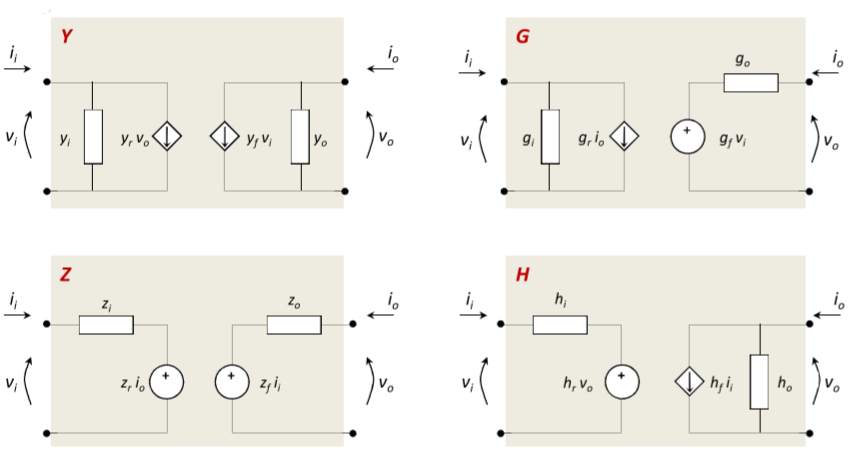
\includegraphics[width=6cm]{img/YZGH.png}
\caption{Les 4 types de quadripoles}
\end{figure}
On peut facilement représenter ces différents systèmes via des matrices détaillants le système
%insérer la matrice

\subsection{L'amplificateur opérationnelle}
L'amplificateur opérationnelle ou \textit{ampli op} est un composant qu'on retrouve abondamment en électronique. 

\subsubsection{Montage inverseur}
\begin{equation}
\frac{v_o}{v_s} ~= -\frac{R_2}{R_1}
\end{equation}

\chapter{Signaux sinusoïdales et phaseurs}
\section{Circuits en régime sinusoïdal}

\subsection{Circuit RC: rappel}
Dans cette partie, on s'intéressera surtout au circuit \textbf{RC}, il est donc bon de rappeler différentes formules:
\begin{align}
I_C(t) &= C \frac{dV_C(t)}{dt}\\
V_R(t) &= RI(t)\\
RC \frac{dV_C(t)}{dt} &= -(V_C(t)-V_S(t))\label{eq:RCsinus}
\end{align}

\begin{figure}[H]
\centering
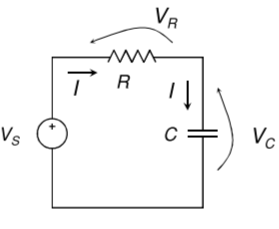
\includegraphics[width=5cm]{img/RCsinus.png} \label{img:RCsinus}
\caption{Circuit RC en régime sinusoïdal}
\end{figure}

Il est à noter que l'équation \ref{eq:RCsinus} est une équation propre au circuit de la figure \ref{img:RCsinus}. Il est bon de remarquer que \textit{maintenant}, les courants et tension sont \textit{dépendantes du temps}. La \textit{constante de temps} est $\tau = RC$ et apparait dans la résolution de \textit{l'équation différentielle}.

\subsection{Circuit LC}
Voici les formules pou les circuits LC. (\textit{note}: on dirait que notre source de courant est une source de courant \textit{commandé} mais c'est bien une source de courant \textbf{non-commandé})
\begin{align}
V_L(t) &= L \frac{dI_L(t)}{dt}\\
V_L(t) &= GI_G(t)\\
GL \frac{dI_L(t)}{dt} &= -(I_L(t)-I_S(t))\label{eq:LCsinus}
\end{align}

\begin{figure}[H]
\centering
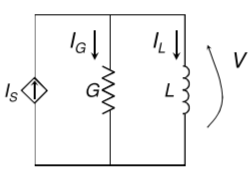
\includegraphics[width=5cm]{img/LCsinus.png} \label{img:LCsinus}
\caption{Circuit LC en régime sinusoïdal}
\end{figure}

Il est à noter que l'équation \ref{eq:LCsinus} est une équation propre au circuit de la figure \ref{img:LCsinus}. La \textit{constante de temps} est $\tau = GL$

\subsection{Régime sinusoïdal}
Quelques notions à bien comprendre:
\begin{itemize}
\item La phase est établi par l'observateur car c'est lui qui définit "\textit{le début de la sinusoïdale}
\item Un cosinus est un sinus \textit{déphasé} de $\frac{\pi}{2}$
\end{itemize}

\subsubsection{Analyse circuit RC}
Si on a une source de courant sinusoïdale:
\begin{align}
V_s(t) &= V_p cos(\omega t)\\
\omega_0 &= \frac{1}{\tau} = \frac{1}{RC}\\
\frac{1}{\omega_0}\frac{dV_c(t)}{dt} + V_c(t) &= V_p cos(\omega t) \label{eq:RCdiff}
\end{align}

L'équation \ref{eq:RCdiff} correspond à l'équation différentielle et à pour solution:

\begin{equation} 
\begin{cases}
V_C(0) = 0\\
V_C(t) = \frac{V_p}{\textcolor{blue}{\sqrt{1 + \frac{\omega^2}{\omega_0^2}}}} \Bigl[\textcolor{brown}{-cos(\phi)e^{-\frac{t}{\tau}}} + \textcolor{green}{cos(\omega t + \phi)} \Bigl] \label{eq:RCsol}
\end{cases} 
\end{equation}
L'équation \ref{eq:RCsol} nous indique plusieurs choses:
\begin{enumerate}
\item La partie en \textcolor{blue}{bleu} nous montre une atténuation du signal.
\item La partie en \textcolor{brown}{brun} nous montre une partie \textit{transitoire} dû à la capacité qui se charge doucement avant d'arriver à un état stable.
\item La partie en \textcolor{green}{vert} est le \textit{déphasage} du signal qui est créé par le caractère "\textit{dérivateur}" d'une capacité
\end{enumerate}

%finir de clarifier les 2 dernières slides de cette sous-section

\subsection{Les Phaseurs}
On utilise des phaseurs pour des circuits \textit{linéaires}, ne possédant \textit{qu'une source indépendante}, on a une source de fréquence $\omega/ 2\pi$ et le circuit est \textit{en régime}.



\end{document}


